%%%%%%%%%%%%%%%%%%%%%%%%%%%%%%%%%%%%%%%%%%%%%%%%%%%%%%%%%%%%%%%%%%%%%%%%%%%%%%%%%%%%%%%%%%%%%
%%									subsection Algorithmes	de Redistribution						%
%%%%%%%%%%%%%%%%%%%%%%%%%%%%%%%%%%%%%%%%%%%%%%%%%%%%%%%%%%%%%%%%%%%%%%%%%%%%%%%%%%%%%%%%%%%%%
\subsection{Algorithme de Redistribution }
 
Après l'envoi des valeurs calculées, les états \emph{Border et Notifier} présentent les valeurs calculées aux paramètres $\parametretwo{}$ et $\parametretree{}$ par la machine locale et les machines distantes. Ces valeurs permettent d'appliquer une stratégie de redistribution des états. La stratégie adoptée est celle d'un jeux non coopératif. Chaque machines cherche a optimisée le temps de calcul de la vérification d'une formule en se focalisant sur l'information que pressente les valeurs calculées par chaque machine. Ainsi, grâce à ces valeurs, sur une machine est calculé calcule l'ensemble minimal des états à envoyer sur une machine distante ainsi que l'ensemble minimal des états à recevoir par cette machine locale. L'envoi des états nécessite la prise en compte de l'équilibrage de charge.  
Dans ce qui suit nous proposons une stratégie de recherche de ces ensembles minimaux d'états à déplacer, dans un sens ou dans l'autre, suivi d'une technique d'envoi de ces ensembles d'états.

L'algorithme de redistribution de l'espace d'états est décrit par l'algorithme \ref{alg6}.\\
\begin{algorithm}[H]
	\SetAlgoLined
	Recherche de l'ensemble minimal des états à deplacer sur une machine distante\; 
	Recherche de l'ensemble minimal des états à deplacer sur la machine locale\; 
	Appliquée une heristique de redistribution sur les deux ensembles\;
	\caption{Distribute State}\label{alg6}
\end{algorithm}
Dans les sections suivantes, nous détaillons les phases de cet algorithme.

\mysubsection{Recherche de l'ensemble minimal des états à deplacer sur une machine distante}{
Dans cette partie l'algorithme cherche parmis les valeurs des paramètres $\parametretwo{}$ et $\parametretree{}$  calculées par les machines distantes le couple minimal. Le nombres des états associés à ce couple doit être inférieur au nombre des états associés au couple calculé par la machine locale. Le déplacement de ces états sur une machine distante permet de diminuer le temps de la vérification car l'algorithme pourra détecter la valeur logique de la formule sur ces états sans qu'une notification ne soit envoyée. Ainsi, le couple minimal est recherché sur les valeurs envoyées par les machines distantes au niveau des états \bn{}, comparées aux valeurs  calculées par la machine locale sur cet état. La recherche du couple minimal est faite en premier temps sur les états ayant une dépendance mutuelle (c'est-à-dire les états distants dépendant l'un de l'autre) car le regroupement de ces états sur une machine diminue le nombre d'itérations de deux. Ainsi, lorsqu'il n'existe pas une dépendance mutuelle entre les états le couple minimum est recherché parmis les valeurs envoyées par les machines distantes au niveau des états \bn{}. La formalisation de ce principe est la suivante: 
\begin{function}

\setcounter{AlgoLine}{0}
\SetKwInOut{MG}{$MG$}
\SetKwInOut{Border}{$Border(F)$}
\SetKwInOut{Notifier}{$Notifier(F)$}
\SetKwInOut{F}{$F$}
\SetKwInOut{ebeta}{$e.\parametretwo{}$}
\SetKwInOut{egama}{$e.\parametretree{}$}
\SetKwInOut{esitebeta}{$e.sites[j].\parametretwo{}$}
\SetKwInOut{esitegama}{$e.sites[j].\parametretree{}$}
\SetKwInOut{e}{$e,e'$}
\SetKwInOut{esite}{$e.site$}
\SetKwInOut{esitej}{$e.site[j]$} 
  \F{} 
\e{}
\ebeta{}
\egama{}
\esite{}
\esitej{}
\esitebeta{}
\esitegama{}
\MG{}
\Border{}
\Notifier{}


\Begin{
	 $MG\longleftarrow null$\;\label{lineI0}\\
\nl	  \ForEach{$e\in \; Border(F)$}{ \label{linerI1}
					\ForEach{$e'\in \; Notifier(F) $}{\label{linerI2}
			\For{$j=1$ \KwTo $size(e'.site)$}{\label{linerI3}
				\If{($(e\in e'.f) and (exist(e.site[j]))and(e.\parametretwo{}>e.site[j].\parametretwo{}) 
					and$\;$ ((e'.\parametretwo{}>e'.site[j].\parametretwo{})or(e'.\parametretwo{}==e'.site[j].\parametretwo{} and e'.\parametretree{}>e'.site[j].\parametretree{})) and$\; $(((MG.\parametretwo{}>e'.site[j].\parametretwo{})or(MG.\parametretwo{}==e'.site[j].\parametretwo{}\; and\; MG.\parametretree{}>e'.site[j].\parametretree{})or \;MG ==null)$) 
					)}{\label{linerI4}
					$MG\longleftarrow e'.site[j]$\;\label{linerI5}
				}
			}
								
		}
	}
	\If{$MG==null$}{\label{linerI6}
		\nl\ForEach{$e\in \; \{Border(F)\cup Notifier(F)\}$}{\label{linerI7}
			\ForEach{$site\in e.site $}{\label{linerI8}
				\If{$((e.\parametretwo{}>site.\parametretwo{} )or (e.\parametretwo{}==site[j].\parametretwo{}\; and\; e.\parametretree{}>site.\parametretree{} )) and(MG ==null or ((MG.\parametretwo{}>site.\parametretwo{} )or \;(MG.\parametretwo{}==site[j].\parametretwo{} \;and\; e.\parametretree{}>site.\parametretree{} )))$}{\label{linerI99}
					$MG\longleftarrow e'.site[j]$\;\label{linerI9}
				}
				
			}	   	
		}\label{linerI10}
	}	 	
	\nl \Return MG\label{linerI11} 
}
	\caption{$Search\_ Min\_ States\_DeplaceOnDistantMachine$():state}
\end{function}


Les instructions décrivant la fonction précédente sont expliquées comme suit:
\begin{description}
	\item[ligne \ref{lineI0} :] L'instruction de cette ligne sert à initialiser la variable stockant les informations du couple minimal.
	\item[ligne \ref{linerI1} :] Parcourir les états \s{\border{}} sur lesquels la formule n'es pas vérifiée. Ainsi, pour chaque état parcouru, les états \s{\notifier} sont parcourus à la ligne \ref{linerI2} pour rechercher le couple minimal parmis les valeurs envoyées par les machines distantes au niveau des états en dépendance mutuelle. Le parcours des valeurs envoyées par les machines distantes est fait à la ligne \ref{linerI3}. Ainsi la vérification du couple minimal est faite  à la ligne \ref{linerI4}. Lorsqu'un couple minimal est trouvé le contenue de la variable \s{MG} est alors remplacé par les informations du nouveau couple (ligne \ref{linerI5}).
	\item[ligne \ref{linerI6} :]  L'instruction de cette ligne vérifie qu'aucun minimum n'a été trouvé lors de la recherche précédente. Lorsque la condition est vérifiée les instructions de la ligne \ref{linerI7} jusqu'à la ligne \ref{linerI10} sont alors exécutées.
	\item[ligne \ref{linerI7} :] L'instruction de cette ligne permet de parcourir les états \s{\bn{}} sur lesquels la formule n'es pas vérifiée.
	\item[ligne \ref{linerI8} :]  Pour chaque état, l'instruction de cette ligne parcoure les valeurs calculées par les machines distantes et recherche le couple minimum. La vérification du minimum est faite à la ligne \ref{linerI99}. Ainsi la vérification de cette condition entraine l'exécution de l'instruction de la ligne \ref{linerI9}, cela permet à remplacer l'ancien couple par le nouveau.
	\item[ligne \ref{linerI11} :] L'instruction écrite sur cette ligne permet de retourner les informations du couple minimal.
\end{description}


\nopagebreak
}

\mysubsection{Recherche de l'ensemble minimal des états à déplacer}{
L'ensemble minimal des états à déplacer dans une machine locale correspond au couple minimum des couples($\parametretwo{}$ et $\parametretree{}$) calculés par la machine locale sur les états(\bn{}). Les états associés à ce couple entrainent un léger déséquilibre qui pourrait être accepté avec l'écart  calculé. La recherche de ce couple ($\parametretwo{}$ et $\parametretree{}$) est formalisée comme suit:


\begin{function}
\setcounter{AlgoLine}{0}

\Begin{
  \nl $MF \longleftarrow null$\;\label{linerD0}\\
  \nl\ForEach{$e\in \; \{Border(S)\cup Notifier(S)\}-\{MG\}$}{ \label{linerD1}
  \nl		\uIf{$(MG==null )$ }{\label{linerD2}
  \nl				\ForEach{$site \in x.site$}{\label{linerD3}
  \nl					\If{$((x.\parametretwo{}<site.\parametretwo{} )or (x.\parametretwo{}==site.\parametretwo{}\; and\; (x.\parametretree{}<site.\parametretree{} )) and(MF ==null \;or\; ((MF.\parametretwo{}>x.\parametretwo{} )\;or (MF.\parametretwo{}==x.\parametretwo{} \; and\; MF.\parametretree{}>x.\parametretree{} )))$}{\label{linerD4}
  \nl						$MF\longleftarrow x$\;\label{linerD5}
  					}	
  				}\label{linerD7}
  			}
\nl  			 \Else{\label{linerD6}
 \nl 			 	$site\longleftarrow findById(MG.id,x.site)$\;\label{linerD7}\\
  \nl			 	\If{$((site \ne null) and((MF==null) or (MF.\parametretwo{}>x.\parametretwo{}) or (MF.\parametretwo{}==x.\parametretwo{} and MF.\parametretree{}>x.\parametretree{})) and ((x.\parametretwo{}<site.\parametretwo{}) or (x.\parametretwo{}==site.\parametretwo{} and x.\parametretree{}<site.\parametretree{})) $}{\label{linerD8}
\nl  			 	$MF\longleftarrow x$\;\label{linerD9}
  			 	}			  			 
 \nl 			 }\label{endD}
   		} 	
   \nl\Return MF\label{linerD10} 	
}
\caption{$Search\_ Min \_ States\_ DeplaceOnLocaleMachine(MG:state): State$}\label{Search1}
\end{function}
Les instructions décrivant la fonction \ref{Search1} sont expliquées comme suit:
\begin{description}
	\item[ligne \ref{linerD0} :] L'instruction de cette ligne sert à initialiser la variable stockant les informations du couple minimum.
	
	\item[ligne \ref{linerD1} :] L'instruction de cette ligne permet de parcourir les états \s{\bn{}} sur lesquels la formule n'es pas vérifiée. L'état dont il est possible d'importer ses successeurs ou prédécesseurs à partir d'une machine distante est exclu du parcours.
	\item[ligne \ref{linerD2} :]  L'instruction de cette ligne vérifie qu'il n'existe pas des états à importer. La vérification de cette condition entraine l'exécution des instructions de la ligne \ref{linerD3} jusqu'à la ligne \ref{linerD7}.
	
	\item[ligne \ref{linerD3} :] L'instruction de cette ligne permet de parcourir les valeurs calculées par les machines distantes, ainsi les comparer avec les valeurs calculées par la machine locale, la comparaison est effectuée à la  ligne \ref{linerD4}. Lorsque les valeurs de la machine locale sont minimales l'instruction de la ligne \ref{linerD5}  est exécutée, elle permet de mettre à jours le couple minimal.
	
	\item[ligne \ref{linerD6} :] Lorsqu'il existe des états à déplacer sur une machine distante, un ensemble des états est alors recherché sur la machine locale pour l'envoyer sur la machine distante. La recherche de ce couple minimal est faite de la ligne \ref{linerD7} jusqu'à la ligne \ref{endD}.
	
	\item[ligne \ref{linerD7} :] L'instruction de cette ligne permet de récupérer sur l'état les valeurs envoyées par la machine distante. Les valeurs sont récupérées lorsque l'identité de la machine existe sur l'ensemble des machines de l'état.
	
	\item[ligne \ref{linerD8} :]  L'instruction de cette ligne vérifie l'existence des valeurs de la machine distante et leurs supérioritées à celle calculées par la machine locale sur cet état. Lorsqu'elles sont inférieurs au minimum  courant, l'instruction de la ligne \ref{linerD9} met à jour le contenu de la variable \s{MF} par ce couple.
	
	\item[ligne \ref{linerD10} :] L'instruction écrite sur cette ligne permet de retourner les informations du couple recherché.
\end{description}
\nopagebreak
}

\mysubsection{Heristique de redistribution de l'espace d'états}{
Après la recherche de l'ensemble minimal des états à déplacer, l'ensemble d'etats peut être déplacer lorsque l'équilibre peut être assurer entre les machines avec une faible duplication des états. Ainsi, le processus de vérification de l'équilibrage de charge est décris comme suit.

\begin{itemize}
 \item  Lorsque le résultat de la différence entre le nombre des états à déplacer et le nombre des états à importer  est inférieur ou égale à l'écart calculé la requête envoyée comporte alors les états migrants de la machine locale et une demande des états de la machine distante.
 \item Sinon, si le nombre des états à déplacer est inférieur ou égale à l'écart calculé la requête comporte les états à insérer sur la machine distante.
 \item Sinon, s'il s'agit des états de la machine distante, la requête concerne ces états afin que la machine distante puisse les envoyer à la machine.
 \end{itemize}  
Ce principe est formalisé comme suit:

\begin{procedure} [H]
	\setcounter{AlgoLine}{0}
  	\Begin{	
  		\nl \uIf{$\mid MG.site.\parametretwo{} -MF.\parametretwo{} \mid \leq \parametrefive{}$}{\label{pline1}
  		\nl	$send(element(MF),MG) to  MG.id$\;\label{pline2}
  		}
  		\nl \uElseIf{$MG.site.\parametretwo{} \leq \parametrefive{}$}{\label{pline3}
  		\nl	$send(null,MG)  to MG.id$\;\label{pline4}
  		}
  		\nl \ElseIf{$MF.\parametretwo{} \leq \parametrefive{}$}{\label{pline5}
  		\nl	$send(element(MF),null)  to  MF.id$\;\label{pline6}
  		}
  	}
\caption{$Send\_ Request(MG:state,MF:state)$}
\end{procedure}
Les instructions décrivant la procédure ($Send\_ Request$) sont expliquées comme suit:
\begin{description}
\item[ligne \ref{pline1} :] L'instruction de cette ligne permet de vérifier qu'il est possible de déplacer des états locaux et des états distants. La vérification de cette condition permet d'exécuter l'instruction de la ligne \ref{pline2}, elle permet d'envoyer les états à déplacer et la référence des états à importer. 
\item[ligne \ref{pline3} :] L'instruction de cette ligne permet de vérifier qu'il est possible de déplacer des états distants. La vérification de cette condition permet d'exécuter l'instruction de la ligne \ref{pline4}, elle permet d'envoyer la référence des états à déplacer à la machine distante. 
\item[ligne \ref{pline1} :] L'instruction de cette ligne permet de vérifier qu'il est possible de déplacer des états locaux. La vérification de cette condition permet d'exécuter l'instruction de la ligne \ref{pline2}, elle permet d'envoyer l'ensemble des états à la machine distante. 
\end{description}

\begin{function}
	\setcounter{AlgoLine}{0}
\Begin { 
 \nl 		$states \leftarrow \emptyset$\;	
\\ \nl 		\uIf{$ type(s) ==border$}{
\nl 			\ForEach {$e' \in S$}{
\nl				\If{$s.f\in e'.f \;$}{
\nl					$states \leftarrow states \cup \{ e'\}$\;	
 			      }
\nl 			\ElseIf{$s.f\in e'.limit$}{
\nl 					$states\leftarrow states \cup \{ e'\}$\;\\	
\nl 					duplicate(e') in this machine\;	
 				}
			}
 		}
\nl 		\ElseIf{$e \; \in notifier(S)$}{
\nl			$states\leftarrow getSucc(s)$\;
			\ForEach {$e' \in e.f$}{
\nl 				\uIf{$type(e) \ne border$}{
\nl 					$states\leftarrow states \cup \{ duplicate(e)\}$\;
 				}
\nl 				\Else{
\nl 					$states\leftarrow states \cup \{ e\}$\;
 				}
 			}
 		} 		  		
}
\caption{$element(s:state)$}
\end{function}


\nopagebreak\nopagebreak\nopagebreak
}
\mysubsection{Réception des états ou la demande des états à deplacer}{
A la réception d'une requête les états à insérer sont insérés et les ensemble des états demandés sont envoyés. Lorsque des états sont insérés à la structure de Kripke d'une machine, les valeurs calculées par la machine distante sont alors mises à jour par celles correspondantes à la machine locale pour le bon fonctionnement du protocole. Après ce processus  l'Algorithme \ref{alg6} est relancé. 
Ce principe est formalisé comme suit:
\SetKwFunction{printlcs}{$Receive\_ Request$}
\begin{algorithm}
 \SetAlgoLined\DontPrintSemicolon
  \SetKwFunction{algo}{\printlcs{states :List of State,MG:State}}\SetKwFunction{proc}{proc}
  \SetKwProg{myalg}{Procedure}{}{}
  \myalg{\algo{}}{ 	
  		\If{$size(states)\ne 0$}{\label{prline1}
  			add(states) in  Sj \;\label{prline2}
  		}
  		\If{$MG\ne null)$}{\label{prline3}
  			$send(element(MG),null)  to MG.id$\;\label{prline4}
  		}
  		algorithm \ref{alg6}()\;\label{prline6}
}{}
\end{algorithm}

Les instructions décrivant la procédure ($Receive\_ Request$) sont expliquées comme suit:
\begin{description}
\item[ligne \ref{pline1} :] L'instruction de cette ligne vérifie que des états ont été  envoyés. La vérification de cette condition permet d'exécuter l'instruction de la ligne \ref{prline2}, elle permet de rajouter les états reçus à la structure de Kripke(ligne \ref{pline2}). 
\item[ligne \ref{pline3} :] L'instruction de cette ligne vérifie qu'une demande concernant un ensemble des états a été envoyé. La vérification de cette condition permet d'envoyer l'ensemble des états concernant la demande (ligne \ref{pline4}). 
\item[ligne \ref{pline5} :] L'instruction sur cette ligne permet de relancer le protocole de redistribution afin de rechercher un ensemble des états à déplacer.   
\end{description}
\nopagebreak
}
\begin{Exemple}\label{ea5}
L'exécution du protocole de redistribution sur les résultats générés dans les exemples précédents permet d'obtenir  les résultats suivants:

\begin{description}
\item[Itération 1 :] Pendant la première itération du protocole sur la \mone{}, l'algorithme détecte que les état \s{S7} et \s{S9} sont mutuellement dépendants. Ainsi, les valeurs envoyées par la \mtwo{} sur l'état \s{S7} sont minimales, les états concernant ces valeurs sont à déplacer de la \mtwo{}. Ainsi les états à déplacer de la \mone{} vers la \mtwo{} sont recherchés, l'algorithme détecte que les états liés à l'état \s{S11} sont minimaux. Les états de cet ensemble sont à envoyer sur la \mtwo{}. Après ces deux processus de recherche, les valeurs sont évaluées afin de ressortir la requête à envoyer. L'évaluation montre qu'il est possible d'importer les prédécesseurs de l'état \s{S7} et les prédécesseurs de  l'état \s{S11}.
L'état \s{s2} ne sera pas envoyé parmi les états à déplacer car la \mtree{} possède des prédécesseurs directs de cet état. Après l'envoi des états à déplacer, la \mone{} possède l'état \s{S9}, quant à l'état \s{S1} il est possédé par la \mtwo{}.


Sur la \mtree{} l'algorithme détecte qu'il est possible de déplacer l'état \s{S22} sur la \mtwo{}.
   Après ces redistributions d'états, le protocole détecte qu'il est impossible de redistribuer les états car il risque d'avoir un déséquilibre de charge sur les machines.
   
\end{description}
\centering
	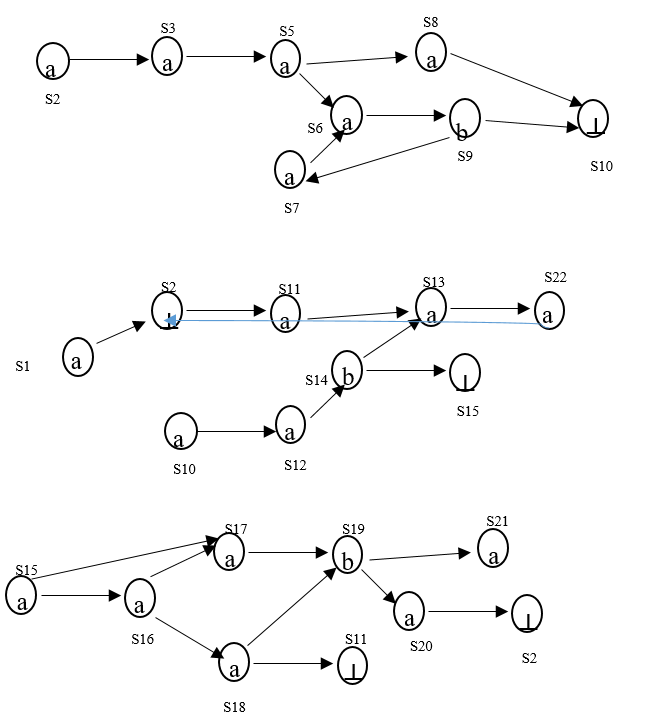
\includegraphics[height=5in]{img/Rskd.png}
	
	\captionof{figure}{Structure de kripke Redistribu\'{e}} 
\end{Exemple}